\documentclass{report}
\usepackage[T1]{fontenc} % Fontes T1
\usepackage[utf8]{inputenc} % Input UTF8
\usepackage[backend=biber, style=ieee]{biblatex} % para usar bibliografia
\usepackage{csquotes}
\usepackage[portuguese]{babel} %Usar língua portuguesa
\usepackage{blindtext} % Gerar texto automaticamente
\usepackage[printonlyused]{acronym}
\usepackage{hyperref} % para autoref
\usepackage{graphicx}
\usepackage{indentfirst}
\graphicspath{{imagens/}}
\bibliography{bibliografia.bib}

\begin{document}

%%
% Definições
%
\def\titulo{Misturador de Músicas}
\def\data{15/06/2018}
\def\autores{André Alves, Daniel Correia, Pedro Almeida, Pedro Valente}
\def\autorescontactos{(88811) andr.alves@ua.pt, (88753) dcorreia@ua.pt,\\
 (89205) pedro22@ua.pt, (88858)pedro.valente@ua.pt}
\def\departamento{Departamento de Electrónica, Telecomunicações e Informática}
\def\empresa{Universidade De Aveiro}
\def\logotipo{img/ua.pdf}
%

%%%%%% CAPA %%%%%%
%
\begin{titlepage}

\begin{center}
%
\vspace*{50mm}
%
{\Huge \titulo}\\ 
%
\vspace{10mm}
%
{\Large \empresa}\\
%
\vspace{10mm}
%
{\LARGE \autores}\\ 
%
\vspace{30mm}
%
\begin{figure}[h]
\center
\includegraphics{\logotipo}
\end{figure}
%
\vspace{30mm}
\end{center}
%

\end{titlepage}

%%  Página de Título %%
\title{%
{\Huge\textbf{\titulo}}\\
{\Large \departamento\\ \empresa}
}
%
\author{%
    \autores \\
    \autorescontactos
}
%
\date{\data}
%
\maketitle

\pagenumbering{arabic}


\tableofcontents
\listoffigures    % descomentar se necessário



\chapter{Introdução}
\label{chap.introducao}
O projeto final da disciplina de Laboratórios de Informática consiste na criação de um sistema de que permite criar músicas através de excertos de música.


	



\chapter{Desenvolvimento}
\label{chap.desenvolvimento}
	
\section{Interface Web}s
..............

\section{Aplicação Web}
................

\section{Persistência}
...............

\section{Gerador de Músicas}
...................



	\begin{figure} [t]
		\centering
		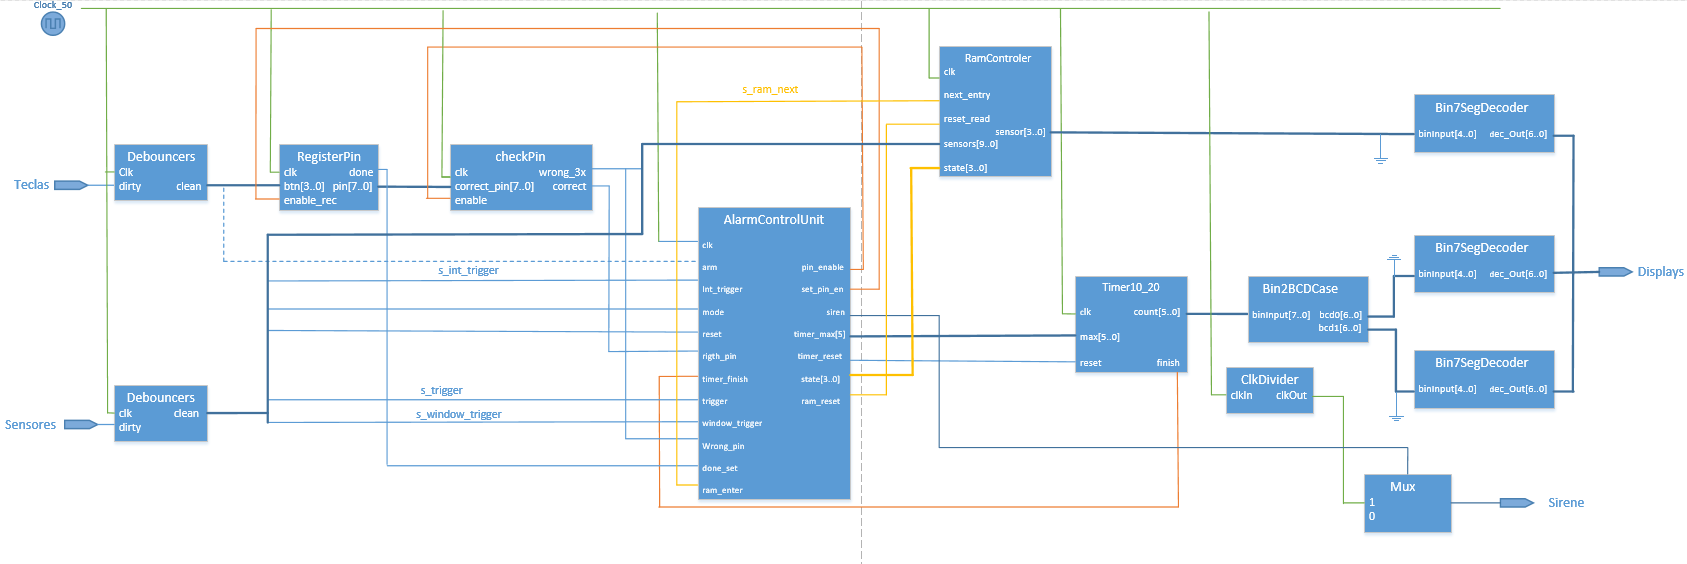
\includegraphics[scale=0.6, angle = 90]{img/arq_final.PNG}
		\caption{Arquitetura geral}
	\end{figure}

	\begin{figure} [h]
		\centering
		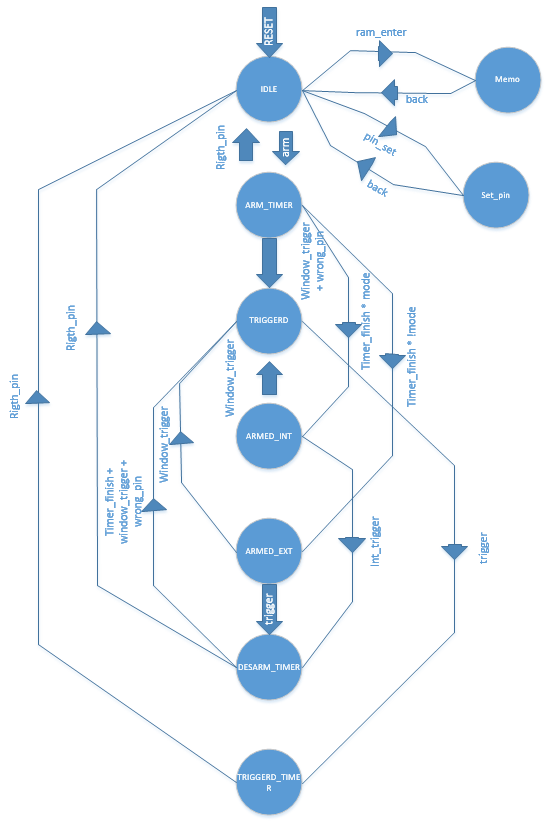
\includegraphics[scale=0.7]{img/m_estados.PNG}
		\caption{Máquina de Estados}
	\end{figure}	
	 

	
\chapter{Conclusões Finais}
\label{chap.conclusao}
	Com este projeto de gerador de músicas foi possível consolidar os conhecimentos adquiridos em aulas pois foi necessário tudo o que foi realizado ao longo semestre.  

 
\chapter{Contribuições dos autores}
\label{contribuições}

\noindent
André Alvez - 10\% \\
Daniel Correia - 75\% \\
Pedro Almeida - 5\% \\
Pedro Valente - 10\% 


\end{document}
